% Notes de cours pour ACT-2005
% Automne 2018
\documentclass[12pt, french]{report}

% Lien vers un template de préambule
% !TEX encoding = UTF-8 Unicode
% LaTeX Preamble
% Author : Gabriel Crépeault-Cauchon
% Last update : 07/10/2018

% HOW-TO : copy-paste this file in the same directory as your .tex file, and add in your preamble the next command right after you have specified your documentclass : 
% % !TEX encoding = UTF-8 Unicode
% LaTeX Preamble
% Author : Gabriel Crépeault-Cauchon
% Last update : 07/10/2018

% HOW-TO : copy-paste this file in the same directory as your .tex file, and add in your preamble the next command right after you have specified your documentclass : 
% % !TEX encoding = UTF-8 Unicode
% LaTeX Preamble
% Author : Gabriel Crépeault-Cauchon
% Last update : 07/10/2018

% HOW-TO : copy-paste this file in the same directory as your .tex file, and add in your preamble the next command right after you have specified your documentclass : 
% \input{preambule_utf8.tex}

% ---------------------------------------------
% BEGINNING OF PREAMBLE
% ---------------------------------------------
% Encoding packages
\usepackage[utf8]{inputenc}
\usepackage[T1]{fontenc}
\usepackage{babel}
\usepackage{lmodern}

% HYPERREF (URL's and Link options)
\usepackage{hyperref}
\hypersetup{colorlinks = true, urlcolor = blue, linkcolor = red!60!black}

% POLICY (choose one of them)
%	\usepackage{concrete}
%	\usepackage{mathpazo}
%	\usepackage{frcursive} %% permet d'écrire en lettres attachées
 \usepackage{aeguill}
% 	\usepackage{mathptmx}
%	\usepackage{fourier} 

% Mathematics configuration
\usepackage{amsmath,amsthm,amssymb,latexsym,amsfonts}
\usepackage{empheq}
\usepackage{numprint}
\usepackage{dsfont} 


% Tcolorbox config
\usepackage{tcolorbox}
\tcbuselibrary{xparse}
\tcbuselibrary{breakable}
%% Définition Boite pour exemple
\newcounter{ex}[section]
\DeclareTColorBox{exemple}{ o }% #1 parameter
{colframe=green!20!black,colback=green!5!white, % color of the box
breakable, pad at break*=0mm, % to split the box
before title = {\textbf{Exemple \stepcounter{ex} \arabic{chapter}.\arabic{section}.\arabic{ex} }},
IfValueTF = {#1}{title= {#1}}{title= \hphantom},
after title = {\large \hfill \faWrench}
}

%% Définition boite pour définition
\newcounter{def}[section]
\DeclareTColorBox{definition}{ o }% #1 parameter
{colframe=blue!60!green,colback=blue!5!white, % color of the box
breakable, pad at break*=0mm, % to split the box
before title = {\textbf{Définition \stepcounter{def} \arabic{chapter}.\arabic{section}.\arabic{def} }},
title = {#1},
after title = {\large \hfill \faBook}
}


% Graphics and picture import Packages
\usepackage{graphicx}
\usepackage{pict2e}

% insert PDF package
\usepackage{pdfpages}

% Color package
\usepackage{color, soulutf8, colortbl}

% usefull shortcut for colored text
\newcommand{\orange}{\textcolor{orange}}
\newcommand{\red}{\textcolor{red}}
\newcommand{\cyan}{\textcolor{cyan}}
\newcommand{\blue}{\textcolor{blue}}
\newcommand{\green}{\textcolor{green}}
\newcommand{\purple}{\textcolor{magenta}}
\newcommand{\yellow}{\textcolor{yellow}}

% Custum enumerate & itemize Package
\usepackage{enumitem}
% French Setup for itemize function
\frenchbsetup{StandardItemLabels=true}

% Mathematics shortcut
\usepackage{cancel}
\newcommand{\reels}{\mathbb{R}}
\newcommand{\entiers}{\mathbb{Z}}
\newcommand{\naturels}{\mathbb{N}}
\newcommand{\eval}{\biggr \rvert}
\newcommand{\esp}[1]{\mathrm{E} \left[ #1 \right]} % espérance
\newcommand{\variance}[1]{\mathrm{Var} \left( #1 \right)} % variance
\newcommand{\covar}[1]{\mathrm{Cov} \left( #1 \right)} % variance
\newcommand{\prob}[1]{\Pr \left( #1 \right)} % probabilité entre parenthèses
\newcommand{\laplace}{\mathcal{L}}

% Actuarial notation package
\usepackage{actuarialsymbol}
\usepackage{actuarialangle}

% To indicate equation number on a specific line in align environment
\newcommand\numberthis{\addtocounter{equation}{1}\tag{\theequation}}

% Other shortcut
\newcommand{\p}{\paragraph{}}
\newcommand{\n}{\newline}
\newcommand{\derivee}[1]{\frac{\partial}{\partial #1}}
\newcommand{\indic}[1]{\mathds{1}_{\{ #1 \}}}

% Special symbols package
\usepackage[tikz]{bclogo}
\usepackage{fontawesome}

% Retire l'indentation automatique de Latex
\setlength{\parindent}{0pt}

% ---------------------------------------------
% END OF PREAMBLE
% ---------------------------------------------

% ---------------------------------------------
% BEGINNING OF PREAMBLE
% ---------------------------------------------
% Encoding packages
\usepackage[utf8]{inputenc}
\usepackage[T1]{fontenc}
\usepackage{babel}
\usepackage{lmodern}

% HYPERREF (URL's and Link options)
\usepackage{hyperref}
\hypersetup{colorlinks = true, urlcolor = blue, linkcolor = red!60!black}

% POLICY (choose one of them)
%	\usepackage{concrete}
%	\usepackage{mathpazo}
%	\usepackage{frcursive} %% permet d'écrire en lettres attachées
 \usepackage{aeguill}
% 	\usepackage{mathptmx}
%	\usepackage{fourier} 

% Mathematics configuration
\usepackage{amsmath,amsthm,amssymb,latexsym,amsfonts}
\usepackage{empheq}
\usepackage{numprint}
\usepackage{dsfont} 


% Tcolorbox config
\usepackage{tcolorbox}
\tcbuselibrary{xparse}
\tcbuselibrary{breakable}
%% Définition Boite pour exemple
\newcounter{ex}[section]
\DeclareTColorBox{exemple}{ o }% #1 parameter
{colframe=green!20!black,colback=green!5!white, % color of the box
breakable, pad at break*=0mm, % to split the box
before title = {\textbf{Exemple \stepcounter{ex} \arabic{chapter}.\arabic{section}.\arabic{ex} }},
IfValueTF = {#1}{title= {#1}}{title= \hphantom},
after title = {\large \hfill \faWrench}
}

%% Définition boite pour définition
\newcounter{def}[section]
\DeclareTColorBox{definition}{ o }% #1 parameter
{colframe=blue!60!green,colback=blue!5!white, % color of the box
breakable, pad at break*=0mm, % to split the box
before title = {\textbf{Définition \stepcounter{def} \arabic{chapter}.\arabic{section}.\arabic{def} }},
title = {#1},
after title = {\large \hfill \faBook}
}


% Graphics and picture import Packages
\usepackage{graphicx}
\usepackage{pict2e}

% insert PDF package
\usepackage{pdfpages}

% Color package
\usepackage{color, soulutf8, colortbl}

% usefull shortcut for colored text
\newcommand{\orange}{\textcolor{orange}}
\newcommand{\red}{\textcolor{red}}
\newcommand{\cyan}{\textcolor{cyan}}
\newcommand{\blue}{\textcolor{blue}}
\newcommand{\green}{\textcolor{green}}
\newcommand{\purple}{\textcolor{magenta}}
\newcommand{\yellow}{\textcolor{yellow}}

% Custum enumerate & itemize Package
\usepackage{enumitem}
% French Setup for itemize function
\frenchbsetup{StandardItemLabels=true}

% Mathematics shortcut
\usepackage{cancel}
\newcommand{\reels}{\mathbb{R}}
\newcommand{\entiers}{\mathbb{Z}}
\newcommand{\naturels}{\mathbb{N}}
\newcommand{\eval}{\biggr \rvert}
\newcommand{\esp}[1]{\mathrm{E} \left[ #1 \right]} % espérance
\newcommand{\variance}[1]{\mathrm{Var} \left( #1 \right)} % variance
\newcommand{\covar}[1]{\mathrm{Cov} \left( #1 \right)} % variance
\newcommand{\prob}[1]{\Pr \left( #1 \right)} % probabilité entre parenthèses
\newcommand{\laplace}{\mathcal{L}}

% Actuarial notation package
\usepackage{actuarialsymbol}
\usepackage{actuarialangle}

% To indicate equation number on a specific line in align environment
\newcommand\numberthis{\addtocounter{equation}{1}\tag{\theequation}}

% Other shortcut
\newcommand{\p}{\paragraph{}}
\newcommand{\n}{\newline}
\newcommand{\derivee}[1]{\frac{\partial}{\partial #1}}
\newcommand{\indic}[1]{\mathds{1}_{\{ #1 \}}}

% Special symbols package
\usepackage[tikz]{bclogo}
\usepackage{fontawesome}

% Retire l'indentation automatique de Latex
\setlength{\parindent}{0pt}

% ---------------------------------------------
% END OF PREAMBLE
% ---------------------------------------------

% ---------------------------------------------
% BEGINNING OF PREAMBLE
% ---------------------------------------------
% Encoding packages
\usepackage[utf8]{inputenc}
\usepackage[T1]{fontenc}
\usepackage{babel}
\usepackage{lmodern}

% HYPERREF (URL's and Link options)
\usepackage{hyperref}
\hypersetup{colorlinks = true, urlcolor = blue, linkcolor = red!60!black}

% POLICY (choose one of them)
%	\usepackage{concrete}
%	\usepackage{mathpazo}
%	\usepackage{frcursive} %% permet d'écrire en lettres attachées
 \usepackage{aeguill}
% 	\usepackage{mathptmx}
%	\usepackage{fourier} 

% Mathematics configuration
\usepackage{amsmath,amsthm,amssymb,latexsym,amsfonts}
\usepackage{empheq}
\usepackage{numprint}
\usepackage{dsfont} 


% Tcolorbox config
\usepackage{tcolorbox}
\tcbuselibrary{xparse}
\tcbuselibrary{breakable}
%% Définition Boite pour exemple
\newcounter{ex}[section]
\DeclareTColorBox{exemple}{ o }% #1 parameter
{colframe=green!20!black,colback=green!5!white, % color of the box
breakable, pad at break*=0mm, % to split the box
before title = {\textbf{Exemple \stepcounter{ex} \arabic{chapter}.\arabic{section}.\arabic{ex} }},
IfValueTF = {#1}{title= {#1}}{title= \hphantom},
after title = {\large \hfill \faWrench}
}

%% Définition boite pour définition
\newcounter{def}[section]
\DeclareTColorBox{definition}{ o }% #1 parameter
{colframe=blue!60!green,colback=blue!5!white, % color of the box
breakable, pad at break*=0mm, % to split the box
before title = {\textbf{Définition \stepcounter{def} \arabic{chapter}.\arabic{section}.\arabic{def} }},
title = {#1},
after title = {\large \hfill \faBook}
}


% Graphics and picture import Packages
\usepackage{graphicx}
\usepackage{pict2e}

% insert PDF package
\usepackage{pdfpages}

% Color package
\usepackage{color, soulutf8, colortbl}

% usefull shortcut for colored text
\newcommand{\orange}{\textcolor{orange}}
\newcommand{\red}{\textcolor{red}}
\newcommand{\cyan}{\textcolor{cyan}}
\newcommand{\blue}{\textcolor{blue}}
\newcommand{\green}{\textcolor{green}}
\newcommand{\purple}{\textcolor{magenta}}
\newcommand{\yellow}{\textcolor{yellow}}

% Custum enumerate & itemize Package
\usepackage{enumitem}
% French Setup for itemize function
\frenchbsetup{StandardItemLabels=true}

% Mathematics shortcut
\usepackage{cancel}
\newcommand{\reels}{\mathbb{R}}
\newcommand{\entiers}{\mathbb{Z}}
\newcommand{\naturels}{\mathbb{N}}
\newcommand{\eval}{\biggr \rvert}
\newcommand{\esp}[1]{\mathrm{E} \left[ #1 \right]} % espérance
\newcommand{\variance}[1]{\mathrm{Var} \left( #1 \right)} % variance
\newcommand{\covar}[1]{\mathrm{Cov} \left( #1 \right)} % variance
\newcommand{\prob}[1]{\Pr \left( #1 \right)} % probabilité entre parenthèses
\newcommand{\laplace}{\mathcal{L}}

% Actuarial notation package
\usepackage{actuarialsymbol}
\usepackage{actuarialangle}

% To indicate equation number on a specific line in align environment
\newcommand\numberthis{\addtocounter{equation}{1}\tag{\theequation}}

% Other shortcut
\newcommand{\p}{\paragraph{}}
\newcommand{\n}{\newline}
\newcommand{\derivee}[1]{\frac{\partial}{\partial #1}}
\newcommand{\indic}[1]{\mathds{1}_{\{ #1 \}}}

% Special symbols package
\usepackage[tikz]{bclogo}
\usepackage{fontawesome}

% Retire l'indentation automatique de Latex
\setlength{\parindent}{0pt}

% ---------------------------------------------
% END OF PREAMBLE
% ---------------------------------------------
% % Preamble for code listing
% Please input this file after your main preamble
% Gabriel Crépeault-Cauchon, 2018
% -------------------------------

% Load the package 
\usepackage{listings}

% -------
% Settings for different programming language : 

% VISUAL BASIC FOR APPLICATION (VBA)
\lstdefinestyle{vba}
{
	language = {[Visual] Basic},	
	breaklines = true,
	extendedchars=\true,
	showstringspaces = false,	
	tabsize = 3,
	breaklines = true,
	keywordstyle = \color{blue},
	commentstyle = \color{green!35!black},
	backgroundcolor = \color{gray!20!white},
	stringstyle = \color{red}
}


% R (to be modified : does not work for now.
\lstdefinestyle{SAS}
{
	language=SAS
}




% Information sur le document
\title{Mathématiques actuarielles IARD-1 \\
ACT-2005 \\
Notes de cours}
\author{Gabriel Crépeault-Cauchon \\
Nicholas Langevin}

% Ajout temporaire, à mettre dans le préambule éventuellement
\usepackage{mathrsfs}


% -----------------------------------
% --- DÉBUT DU DOCUMENT ---
\begin{document}

% Page titre
\maketitle

% Table des matières
\tableofcontents

% --- DÉBUT DE LA RÉDACTION ---

% --- RÉSUMÉ ---
\begin{abstract}
Ce document résume les notes de cours prises en classe dans le cours de Mathématiques actuarielles IARD-1, ainsi que des notions prises du livre \textit{LOSS MODELS - From Data to Decisions, 4\up{th} edition}. Il est séparé en 2 parties : la matière qui a été couverte avant et après l'examen partiel. \\

Le chapitre correspondant dans le \emph{Loss Models, 4\up{th} edition} est indiqué entre parenthèse des chapitres. \\

De plus, ce document essaie le plus possible de suivre la numérotation des sections du \emph{Loss Models}. C'est pourquoi il arrive parfois qu'il y ait des sauts de section. \\

Finalement, il y a une section à la fin des chapitres qui indique les exercices recommandés dans le livre, intitulée \textbf{Exercices recommandés}.
\end{abstract}
% --------------


\part{Matière pour l'examen partiel}

\chapter{Quelques rappels de Probabilité}
La loi gamma : 
\begin{align*}
\Gamma(\alpha) = \int_{0}^{\infty} x^{\alpha-1} e^{-x} dx
\end{align*}
De plus, on a
\[\Gamma(\alpha) = (\alpha-1) \Gamma(\alpha-1)\]
et
\[\Gamma(n) = (n-1)!\]

\section{Fonction de survie}
On a
\begin{align*}
\esp{X} & = \int_{-\infty}^{\infty} x f_X(x) dx \\
	& = \int_{-\infty}^{\infty} S_X(x) dx \\
\end{align*}
De plus,
\begin{align*}
f_X(x) = - \derivee{x} S_X(x)
\end{align*}
\begin{proof}
\begin{align*}
f_X(x)	&  =-  \derivee{x} S_X(x)  \\
	&=-  \derivee{x} (1  - F_X(x))  \\
	& = - (- f_X(x)) \\
	& = f_X(x) \\
\end{align*}
\end{proof}





\chapter{Quantités des distributions à connaître (3)}
\section{Moments}

\paragraph{\textit{Raw moments}}
On représente le $k$\up{e} moment par $\mu_k^\prime$, soit
\begin{equation}
\mu_k^\prime = \esp{X^k} 
\end{equation}

\paragraph{Moments centraux} Le $k$\up{e} moment central est représenté par
\begin{equation}
\mu_k = \esp{(X - \mu)^k}
\end{equation}

\begin{exemple}[Quelques exemples de moments centraux]
La variance est le 2\up{e} moment central : 
\begin{align*}
Var(X) = \mu_2 =  \esp{(X - \mu)^2} \\
\end{align*}
Le 3\up{e} moment centré, qui est utilisé pour calculer le coefficient d'asymétrie : 
\begin{align*}
\mu_3 = \esp{(X-\mu)^3}
\end{align*}
\end{exemple}

\paragraph{Coefficient de variation}
\begin{equation}
CV = \frac{\sigma}{\esp{X}}
\end{equation}


\paragraph{Coefficient d'asymétrie}
Le coefficient d'asymétrie, aussi appelé \textit{skewness}, est défini par
% J'ai pris la notation du livre Loss Model pour le skewness.
\begin{equation}
\gamma_1 = \frac{\mu_3}{\sigma^3}
\end{equation}
Soit le 3\up{e} moment standarisé. Si $S_k = 0$, alors la distribution tend vers une loi normale, telle qu'on le voit sur la figure ci-dessous : 

\begin{center}
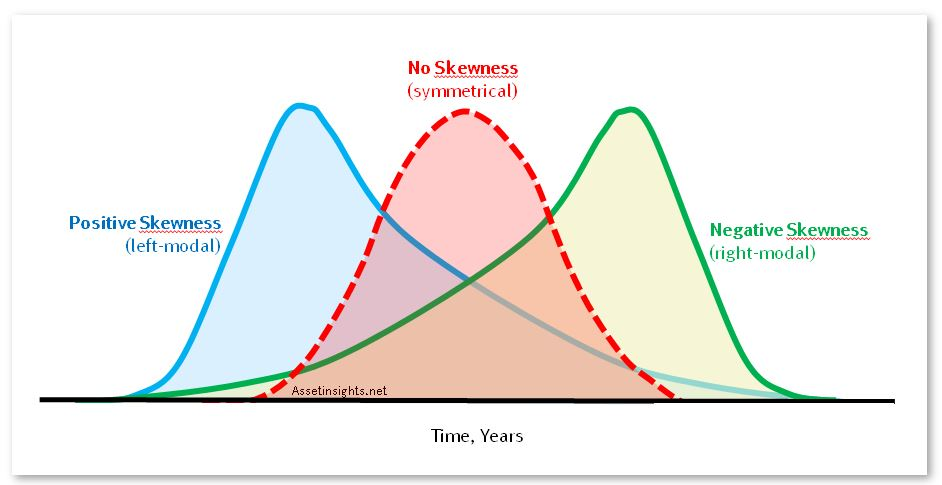
\includegraphics[scale=0.4]{Figures/skewness_interpretation.jpg}
\end{center}

\paragraph{Coefficient d'applatissement}
Le coefficient d'applatissement, aussi appelé \textit{Kurtosis}, se définit par
\begin{equation}
\text{Kurtosis} = \frac{\mu_4}{\sigma^4}
\end{equation}
Cette quantité permet de mesurer l'épaisseur de l'aile (\textit{tail}) de la distribution. Si $\esp{z^4} =3$, alors la distribution tend vers une loi normale $N(\mu, \sigma^2)$.

\paragraph{Mean Excess Loss}
On définit la variable aléatoire $Y^P$, qui représente le montant de perte en excès d'un déductible $d$, sachant que la perte est au delà de ce montant. On peut définir l'espérance des coûts de cette variable alétaoire : 
\begin{equation}
e(d) = \esp{Y^P} = \esp{X-d | X \geq d} = \frac{\int_{d}^{\infty} S_X(x)}{S_X(d)}
\end{equation}

Note : cette variable est dite tronquée à gauche et \textit{shifted}. On entend parfois aussi \textit{Per-payment}
	

\paragraph{Left censored and shifted variable}
Soit la v.a. $Y^L$, qui représente le montant payé par l'assureur \textit{par perte}. La variable est donc dite \textit{censurée à gauche et shifted}. On peut aussi en calculer l'espérance : 
\begin{equation}
\esp{Y^L} = \esp{(X-d)_+} = \int_{d}^{\infty} (x-d) f_X(x) dx
\end{equation}
De plus, on peut facilement déduire la relation suivante : 
\begin{align*}
\esp{(X-d)_+} = e(d) (1 - F_X(d))
\end{align*}

\paragraph{Limited Loss Variable} Finalement, on peut définir la variable $Y$, qui représente le paiement de l'assureur avec une limite de $u$ à la police. Son espérance est définie par
\begin{equation}
\esp{X \wedge u} = \int_{0}^{u} f_X(x) dx
\end{equation}
À l'aide d'intégration par partie, on peut trouver la forme suivante : 
\begin{align*}
\esp{X \wedge u} = \int_{0}^{u} S_X(x) dx
\end{align*}
La v.a. $Y$ est dite \textit{censurée à droite et shifted}

\begin{exemple}[lien entre le déductible et la limite]
On peut faire le lien entre le déductible et la limite : 
\begin{center}
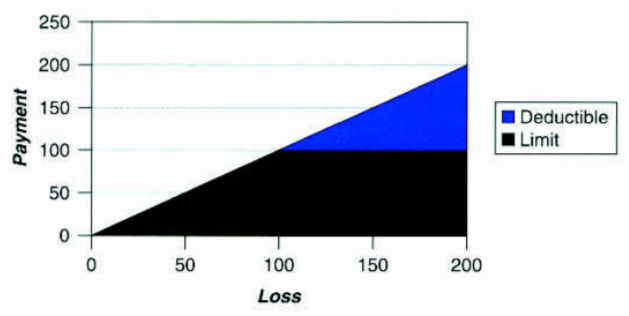
\includegraphics[scale=0.45]{Figures/distinction_loss-deductible-limit}
\end{center}
\end{exemple}

\setcounter{section}{3}
% Ne semble pas pertinent pour l'Examen ...
%\section{La loi normale}
%
%\paragraph{La fonction génératrice des moments}
%\begin{align*}
%    M_x(t) &= M_x(0) + \frac{M_x^\prime t}{1!} + \frac{M_x^{\prime\prime} t^2}{2!} + ... + \frac{M_x^{(n) t^n}}{n!} \\
%           &= 1 + \frac{E[x] t}{1!} + \frac{E[x^2] t^2}{2!} + ... + \frac{E[x^n] t^n}{n!}
%\end{align*}
%
%On pose: $c_k = \frac{E[x^n]}{n!}$ alors,
%
%\begin{equation}
%    E[x^k] = C_k k!
%\end{equation}

\section{Percentile}
\label{sec:percentile}
On définit le $p$\up{e} quantile (\emph{percentile} en anglais) $\pi_p$ comme étant la valeur minimale que $X$ prend tel que $F_X(\pi_p) \geq p$. \\

Il arrive parfois (en contexte où $x$  est discret) que le $p$ percentile demandé tombe dans une \emph{marche}. Il faut alors considérer les bornes de la fonction pour déterminer quelle valeur de $x$ correspond au quantile demandé.


\section{Queue de distribution}
\subsection{Classification selon les moments}
\begin{enumerate}[label=\faAngleRight]
\item On peut déterminer si une distribution a une \textit{heavy-tail} en vérifiant si ses moments existent.

\item On peut aussi comparer des distributions entre-eux en utilisant des quantités standarisées, telles que le Coefficient de variation, le coefficient d'asymétrie (\textit{skewness}) ou encore le coefficient d'applatissement (\textit{Kurtosis})
\end{enumerate}

\subsection{Classification selon les comportements limites des ailes de distribution}
\begin{enumerate}[label=\faAngleRight]
\item On peut faire le ratio de deux distributions avec leurs fonction de survie ($S(x)$) ou leur fonction $f$ de densité pour vérifier laquelle des 2 a la plus grosse aile de distribution (\textit{tail}).

\end{enumerate}

\begin{enumerate}
    \item Sois $f_1(x)$ une fonction tels que les 3 premiers moment existe: $E[x^4] = \infty$
    \item Sois $f_2(x)$ une fonction tels que les 2 premiers moment existe: $E[x^2] = \infty$
\end{enumerate}
Alors,
\begin{align*}
    \lim_{x\to\infty} r(x) = \frac{f_1(x)}{f_2(x)} = \left\{
                                                        \begin{array}{ll}
                                                            \infty ,\: f_1(x) \text{a une aile plus lourde que} f_2(x) \\
                                                            0      ,\: f_2(x) \text{a une aile plus lourde que} f_1(x) 
                                                        \end{array}
                                                    \right.
\end{align*}
\begin{exemple}
    Sois $f_{x_1}(x_1) \sim pareto(\alpha, \theta)$ et $f_{x_2}(x_2) \sim gamma(\alpha, \lambda)$ 
    \begin{align*}
        \lim_{x\to\infty} r(x) &= \lim_{x\to\infty} \frac{f_{x_1}(x_1)}{f_{x_2}(x_2)} \\
                               &= \frac{\frac{\alpha \theta^\alpha}{(x + \theta)^{\alpha + 1}}}{\lambda^\alpha x^{\alpha - 1} e^{-\lambda x}} \\
                               &= C \frac{e^{-\lambda x}}{x^{\alpha - 1} (x + \theta)^{\alpha + 1}} \\
                               &= \infty
    \end{align*}      
    La pareto a une queue plus lourde que la gamma
\end{exemple}


\subsection{Classification basée sur la fonction de Hazard}

\begin{definition}[\textit{Hazard rate function}]
La fonction de hazard (aussi appelée force de mortalité ($\mu(x)$) ou le failure rate ($\lambda(x)$), est définie par
\begin{equation}
h_X(x) = \frac{f_X(x)}{S_X(x)}
\end{equation}
On peut aussi exprimer la fonction $h_X(x)$ comme
\begin{align*}
h_X(x) = - \ln (S_X(x))
\end{align*}
\end{definition}
Soit une distribution ayant fonction de densité $f_X(x)$ et fonction de hazard $h_X(x)$. Alors,
\begin{enumerate}[label=\faAngleRight]
\item Si $h(x) \ \nearrow$, \textit{light-tailed}
\item Si $h(x) \ \searrow$, \textit{heavy-tailed}
\item Note : on peut aussi comparer les distributions entre-elles : si une distribution voit son $h_1(x)$ augmenter plus rapidement que l'autre (i.e. $h_2(x)$), alors la deuxième distribution a une aile de distribution plus lourde.
\end{enumerate}

\section{Exercices recommandés}
À compléter


\chapter{Fréquence et sévérité avec modifications aux contrats (8)}
\setcounter{section}{1}
\section{Déductibles}
\subsection{Ordinary deductible}
\subsubsection{Définition}
Soit un contrat d'assurance avec déductible $d$. Lors d'une perte, l'assureur va payer tout montant en excédent du montant $d$. Alors, pour la variable \textit{per-payment},
\begin{equation}
Y^L = (X-d)_+ = 
\begin{cases}
0		& , X \leq d \\
X - d	& , X > d \\
\end{cases}
\end{equation}

\begin{equation}
Y^P = (X-d)_+ = 
\begin{cases}
\text{Non-défini}		& , X \leq d \\
X - d	& , X > d \\
\end{cases}
\end{equation}

\subsubsection{Fonctions reliées}

Et on peut aussi déduire toutes les fonctions qui y sont reliées : 
\begin{align*}
f_{Y^P}(y) = \frac{f_X(y+d)}{S_X(d)}
\end{align*}

\begin{align*}
S_{Y^P}(y) = \frac{S_X(y+d)}{S_X(d)}
\end{align*}

\begin{align*}
F_{Y^P}(y) = \frac{F_X(y+d) - F_X(d)}{S_X(d)}
\end{align*}

\begin{align*}
h_{Y^P}(y) = h_X(y+d)
\end{align*}

Pour la v.a. $Y^L$ \textit{per-loss}\footnote{Il est à noter que la fonction de Hazard n'est pas définie à 0.},
\begin{align*}
f_{Y^L}(y) = f_X(y+d)
\end{align*}

\begin{align*}
S_{Y^L}(y) = S_X(y+d)
\end{align*}

\begin{align*}
F_{Y^L}(y) = F_X(y+d)
\end{align*}

\subsubsection{Espérance}
\begin{equation}
\esp{Y^L} = \esp{(X-d)_+} = \esp{X} - \esp{X \wedge d}
\end{equation}

\begin{equation}
\esp{Y^P} = \frac{\esp{(X-d)_+}}{S_X(d)} = \frac{\esp{X} - \esp{X \wedge d}}{S_X(d)}
\end{equation}

Cette espérance s'appelle la prime \textit{Stop-Loss}, et elle est définie par
\begin{align*}
E[Y]		& = \esp{(X-d)_+} \\
	& = \int_{d}^{\infty} (x-d) f(x) dx \\
	& = \underbrace{\int_{d}^{\infty} x f(x) dx}_{\text{Intégration par partie}} - d \int_{d}^{\infty} f(x) dx \\
	& = -x S(x) \eval_d^\infty + \int_{d}^{\infty} S(x) dx  - s S(d) \\
	& = 0  \cancel{+ S(d)} +  \int_{d}^{\infty} S(x) dx  \cancel{- S(d)} \\
	& = \int_{d}^{\infty} S(x) dx \\
\end{align*}

\subsection{Franchise deductible}

\subsubsection{Définitions}
Lorsque la perte dépasse le déductible franchise de montant $d$, l'assureur assume l'entièreté des coûts \footnote{On voit plus souvent ce type de déductible dans un contexte d'invalidité : si on est absent plus d'un certain nombre de jours du travail, on se fait rembourser toutes ses absences en salaire.}. Pour la v.a. $Y^L$, on a
\begin{align*}
Y^L = 
\begin{cases}
0		& , X \leq d \\
X		& , X > d \\
\end{cases}
\end{align*}
Pour la v.a. $Y^P$,
\begin{equation}
Y^P = 
\begin{cases}
\text{non-défini}	& X \leq d \\
X	& , X > d \\
\end{cases}
\end{equation}

\subsubsection{Fonctions reliées}
Les fonctions de la v.a. $Y^L$ sont
\begin{align*}
f_{Y^L}(y) = 
\begin{cases}
F_X(d)	& , y = 0 \\
f_X(y)	& , y > 0 \\
\end{cases}
\end{align*}

\begin{align*}
F_{Y^L}(y) = 
\begin{cases}
F_X(d)	& , 0 < y \leq d \\
F_X(y)	& , y \geq d \\
\end{cases}
\end{align*}

\begin{align*}
S_{Y^L}(y) = 
\begin{cases}
S_X(d)	& , 0 < y \leq d \\
S_X(x)	& , y > d \\
\end{cases}
\end{align*}

\begin{align*}
h_{Y^L}(y)	= 
\begin{cases}
h_X(d)	& , 0 < y \leq d \\
h_X(x)	& , y > d \\
\end{cases}
\end{align*}

Pour la fonction $Y^P$ (\textit{per-payment}),
\begin{align*}
f_{Y^P}(y) = \frac{f_X(d)}{S_X(d)}
\end{align*}

\begin{align*}
F_{Y^P}(y)	& = 
\begin{cases}
F_X(d)	& , y = 0 \\
F_X(d)	& , 0 < y \leq d \\
\frac{F_X(y) - F_X(d)}{S_X(d)}	& , y > d \\
\end{cases}
\end{align*}

\begin{align*}
S_{Y^P}(y) = 
\begin{cases}
1	& , 0 \leq y \leq d \\
\frac{S_X(y)}{S_X(d)}	& , y > d \\
\end{cases}
\end{align*}

\begin{align*}
h_{Y^P}(y) = 
\begin{cases}
0		& , 0 < y \leq d \\
h_X(y)	& , y > d \\
\end{cases}
\end{align*}

\subsubsection{Espérance}
\begin{equation}
\esp{Y^L} = \esp{(X-d)_+^F} = \esp{X} - \esp{X \wedge d} + d S_X(d)
\end{equation}
\begin{equation}
\esp{Y^P} = \esp{(X-d)_+^F} = \frac{\esp{X} - \esp{X \wedge d}}{S_X(d)} + d
\end{equation}

\section{Loss Elimination Ratio}
\begin{definition}[Loss Eliminating Ratio]
Le Loss Eliminating Ratio ($LER$), nous permet d'obtenir le pourcentage de perte qu'on ne paiera pas grâce au déductible $d$ : 
\begin{align*}
LER 	& = \frac{\esp{X} - \esp{(X-d)_+}}{\esp{X}} \\
\shortintertext{Mais on sait que}
\esp{(X-d)_+}	& = \esp{X} - \esp{X \wedge d} \\
\end{align*}
Alors,

\begin{equation}
LER  = \frac{\esp{X \wedge d}}{\esp{X}} 
\end{equation}
\end{definition}

\paragraph{Note sur l'inflation} Il arrive en exercice qu'on nous demande de comparer ce ratio avec et sans inflation. Soit un contrat avec $r$ $\%$ d'inflation. Alors, on peut trouver $\esp{(X-d)_+}$ qui tient compte de cette inflation : 
\begin{align*}
\esp{(X-d)_+^I} = (1+r) \left( \esp{X} - \esp{X \wedge \frac{d}{1_r}} \right)
\end{align*}

\begin{proof}
\begin{align*}
\esp{Y}	& = (1+r) \int_{\frac{d}{1+r}}^{\infty} x f_X(x) dx - d \int_{\frac{d}{1+r}}^{\infty} f_X(x) dx \\
	\shortintertext{En ajoutant un terme,} \\
	& = \underbrace{(1+r) \blue{\int_{0}^{\frac{d}{1+r}} x f_X(x) dx} + \int_{\frac{d}{1+r}}^{\infty} x f_X(x) dx}_{\esp{X}} - \underbrace{\blue{ \int_{0}^{\frac{d}{1+r}} x f_X(x) dx} - \frac{d}{1+r} \int_{\frac{d}{1+r}}^{\infty} f_X(x) dx}_{\esp{X \wedge \frac{d}{1+r}}} \\ 
	& = \esp{X} - \esp{X \wedge \frac{d}{1+r}} \\
\end{align*}
\end{proof}


\section{Policy Limits}
\subsection{Définitions}
Soit un contrat d'assurance où il est conclu que l'assureur débourse un maximum de $u$ dans le montant de la perte. Ce type de modification au contrat créé une v.a. \textit{censurée à droite}, i.e. le montant déboursé est maximisé à $u$. On définit $Y$ comme étant
\begin{equation}
Y = 
\begin{cases}
X		& , X \leq u \\
u		& , Y > u \\
\end{cases}
\end{equation}

\subsection{Fonctions reliées}
On peut déduire les fonctions reliées suivantes : 
\begin{align*}
f_Y(y) = 
\begin{cases}
f_X(y)	& , y < u \\
S_X(u)	& , y = u \\
\end{cases}
\end{align*}

\begin{align*}
F_Y(y) =
\begin{cases}
F_X(y)	& , y \leq u \\
1	& , y > u \\
\end{cases}
\end{align*}

\paragraph{Note sur l'inflation} Si on a $r$ $\%$ d'inflation, alors
\begin{align*}
\esp{X \wedge u} = (1+r) \esp{X  \wedge \frac{u}{1+r}}
\end{align*}

\begin{proof}
\begin{align*}
\esp{Y}	& = \int_{0}^{\frac{u}{1+r}} (1+r) x f_X(x) dx  + u \int_{\frac{u}{1+r}}^{\infty} f_X(x) dx \\
	& = (1+r) \int_{0}^{\frac{d}{1+r}} f f_X(x) dx + s S_X \left( \frac{u}{1+r} \right) \\
	& = (1+r) \left( \int_{0}^{\frac{u}{1+r}} x f_X(x) dx  + \frac{u}{1+r} S_X \left( \frac{u}{1+r} \right)    \right)	 \\
	& = (1+r) \esp{X  \wedge \frac{u}{1+r}}  \\
\end{align*}
\end{proof}

\section{Coassurance, déductible et limites}
\subsubsection{Définitions}
Le livre nous donne une fonction de perte qui englobe 4 éléments en même temps : l'inflation, les déductibles, la coassurance\footnote{Dans ce type de contrat, la compagnie paie une proportion $\alpha$ de la perte, et le $(1-\alpha)$ restant est assumé par le titulaire de la police.} et les limites de police. Pour la v.a. $Y^L$,
\begin{equation}
Y^L = 
\begin{cases}
0		& ,\ x  < \frac{d}{1+r} \\
\alpha \Big( (1+r) x - d \Big)	& ,\ \frac{d}{1+r} \leq x < \frac{u}{1+r} \\
\alpha (u-d)		& ,\ x \geq \frac{u}{1+r} \\
\end{cases}
\end{equation}
et pour $Y^P$,
\begin{equation}
Y^L = 
\begin{cases}
\text{Non-défini}		& ,\ x  < \frac{d}{1+r} \\
\alpha \Big( (1+r) x - d \Big)	& ,\ \frac{d}{1+r} \leq x < \frac{u}{1+r} \\
\alpha (u-d)		& ,\ x \geq \frac{u}{1+r} \\
\end{cases}
\end{equation}

\subsubsection{Espérance}
\begin{equation}
\esp{Y^L} = \alpha (1+r) \left( \esp{X \wedge \frac{u}{1+r}} - \esp{X \wedge \frac{d}{1+r}}   \right)
\end{equation}
\begin{equation}
\esp{Y^P} = \frac{\esp{Y^L}}{S_X \left( \frac{d}{1+r} \right)}
\end{equation}


% Preuve à retravailler
%\begin{proof}
%On va utiliser $Y = Y_1 - Y_2$ pour prouver. On définit $Y_1$ et $Y_2$ : 
%\begin{align*}
%Y_1	& = 
%\begin{cases}
%0				& , X \leq \frac{d}{1+r} \\
%(1+r)X - d		& , X  > \frac{d}{1+r} \\
%\end{cases} \\
%Y_2	& = 
%\begin{cases}
%0				& , X \leq \frac{u}{1+r} \\
%(1+r) X - u		& , X > \frac{u}{1+r} \\
%\end{cases} \\
%\shortintertext{On connait leur espérance respective,} \\
%\esp{Y_1}	& = (1+r) \left( \esp{X} - \esp{X \wedge \frac{d}{1+r}} \right) \\
%\esp{Y_2}	& = (1+r) \left(\esp{X} - \esp{X \wedge \frac{u}{1+r}} \right) \\
%\shortintertext{Alors,}
%\esp{Y}		& = \esp{Y_1} - \esp{Y_2} \\
%			& = (1+r) \left( \esp{X \wedge \frac{u}{1+r}} - \esp{X \wedge \frac{d}{1+r}}  \right) \\
%\end{align*}
%\end{proof}

\begin{align*}
\esp{Y}	& = \int_{\frac{d}{1+r}}^{\frac{u}{1+r}} ((1+r) x - d) f_X(x) dx + \int_{\frac{u}{1+r}}^{\infty} (u-d) f_X(x) dx \\
	& = (1+r) \left( \esp{X \wedge \frac{u}{1+r}} - \esp{X \wedge \frac{d}{1+r}}   \right) \\
\end{align*}

\section{Exercices recommandés}
À compléter





\chapter{Estimation de données complètes (11)}
\label{chap:estimation_Fn}
\setcounter{section}{1}
% Commence à la section 11.2 dans le Loss Models 4th edition

\section{Estimation de données complètes}
\subsection{Estimation de la fonction de répartition empirique}
On cherche à estimer $F(t)$ ou $S(t)$, lorsque nos données sont complètes (i.e. $x_1, ..., x_n$ qui sont $iid$). Alors, l'estimateur non paramétrique pour $F(t)$ : 
\begin{equation}
F_n(t)	 = \frac{1}{n} \sum_{i=1}^{n} \indic{x_i \leq t}
\end{equation}
où $\indic{.}$ représente une fonction indicatrice.

$F_x(t)$ aura donc la forme suivante : 
\begin{equation}
F_n(t) =
\begin{cases}
0				& , t < x_{(1)} \\
\frac{1}{n}		& , x_{(1)} \leq t < x_{(2)} \\
\frac{2}{n}		& , x_{(2)} \leq t < x_{(3)} \\
...				& \\
1				& , t \geq x_{(n)} \\
\end{cases}
\end{equation}
où $t \in [0, x_{(n)}]$.

\begin{center}
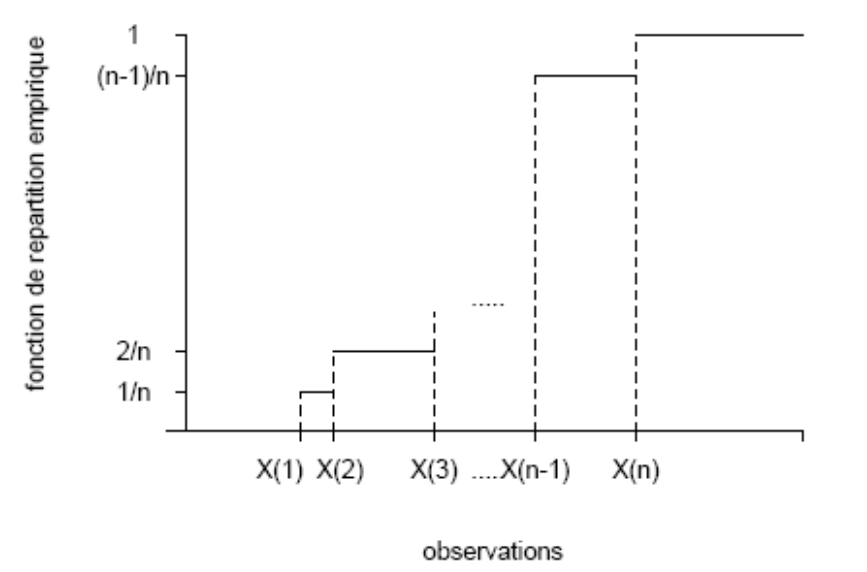
\includegraphics[scale=0.3]{Figures/Fct_de_repartition_empirique}
\end{center}


\paragraph{Remarques}
\begin{enumerate}[label=(\arabic*)]
\item Lorsque $F_n(t) \to F(t)$, alors

\item Puisqu'on a
\begin{align*}
\sum_{i=1}^{n} 1_{[x_i \leq t]} \sim Bin(n,\prob{X \leq t})
\end{align*}
Alors,
\begin{align*}
\esp{F_n(t)}		& = \frac{1}{n} n F(t) \\
	& = F(t) \quad \text{(C'est un estimateur sans biais)} \\
Var \left( F_n(t) \right) & = \frac{1}{n^2}  n F(t) S(t) \\
	& = \frac{F(t) S(t)}{n}	\\
	& \underset{n \to \infty}{=} 0 \\
\end{align*}
\end{enumerate}

\subsection{\textit{Cumulative hazard-rate function}}
On utilise cette fonctoin pour pouvoir réussir à estimer la fonction de densité et le \textit{hazard rate} empirique. En effet, puisque la distribution empirique est discrète, on ne peut pas dériver $F_n(x)$ pour obtenir $f_n(x)$ et $h_n(x)$. La fonction de hazard cumulative se définit par
\begin{equation}
H_X(x) = - \ln S_X(x)
\end{equation}

\subsection{Notation à utiliser pour la distribution empirique}
\begin{enumerate}[label=\faAngleRight]
\item \blue{$y_1 < y_2 < ... < y_k$} : les $k$ valeurs uniques qui apparaissent dans l'échantillon de $n$. \textbf{Note : } $k \leq n$.

\item \blue{$s_j$} : nombre de fois que l'observation $y_j$ est observée dans l'échantillon. On a
\begin{align*}
\sum_{j=1}^{k} s_j = 1
\end{align*}

\item \blue{$r_j$} : nombre d'observations qui sont plus grandes ou égales à $y_j$. On a
\begin{align*}
r_j = \sum_{i=j}^{k} s_i
\end{align*}

\item Avec cette nouvelle notation, on peut ré-écrire la fonction de répartition empirique : 
\begin{equation}
F_n(x) = 
\begin{cases}
0						& , x < y \\
1 - \frac{r_j}{n}		& , y_{j-1} \leq x \leq y_j \quad j = 2, ..., k \\
1						& , x \geq y_k \\
\end{cases}
\end{equation}
\end{enumerate}

\subsection{Estimateur de Nelson \r{A}alen}
\label{subsec:nelson-Aalen}
Pour pouvoir estimer la \textit{Cumulative hazard-rate function}, on doit utiliser un estimateur qui se base sur la notation utilisée à la sous-section précédente, soit le \textit{Nelson \r{A}alen estimate} : 
\begin{equation}
\hat{H}(x) = 
\begin{cases}
0		& , x < y_1 \\
\sum_{i=1}^{j-1} \frac{s_i}{r_i}	& , y_{j-1} \leq x \leq y_j \quad j = 2, ..., k \\
\sum_{i=1}^{k} \frac{s_i}{r_i}		& , x \geq y_k \\
\end{cases}
\end{equation}

\section{Distribution empirique avec données groupées}

\subsection{Fonction OGIVE}
\red{\textbf{CETTE MATIÈRE NE SERA PAS TESTÉE À L'EXAMEN intra A2018}}


%% VOIR SECTION 11.3 dans le livre %%
% Grahique de fonction de répartition empirique à insérer ici
Dans certains contextes, on a $n$ données qui sont groupées en intervalles. La fonction OGIVE permet d'interpoler entre 2 points $c_{j-1}$ et $c_{j}$.
% Graphique des c^(i) et des intervalles n à insérer ici %%
\begin{align*}
c_{j-1} 	 \leq x  \leq c_j \\
F_n(c_{j-1})	 \leq F_n(x)	 \leq F_n(c_j) \\
\end{align*}
On peut déterminer la valeur empirique de $F_n(x)$ aux bornes des classes, avec
\begin{align*}
F_n(x) = \frac{\sum_{i=1}^{j} n_i}{n}
\end{align*}
où $n_i$ est le nombre d'observations qui sont entre $c_{j-1}$ et $c_j$. Toutefois, pour les valeurs entre deux bornes $c_0 < c_1 < ... < c_k$, il faut approximer avec la fonction OGIVE ci-dessous : 

\begin{equation}
\label{eq:repart-OGIVE}
F_n^{\text{OGIVE}}(x) = \frac{c_j - x}{c_j - c_{j-1}} F_n(c_j -1) + \frac{x - c_{j-1}}{c_j - c_{j-1}} F_n(c_j)
\end{equation}



\paragraph{Remarques}
\begin{enumerate}[label=(\arabic*)]
\item Si $x = c_{j-1}$,
\begin{align*}
F_n(c_{j-1}) = F_n^{\text{OGIVE}}(c_{j-1}) \\
\end{align*}
\item Si $x = c_j$,
\begin{align*}
F_n(c_j) = F_n^{\text{OGIVE}}(c_j)
\end{align*}

\item En dérivant \eqref{eq:repart-OGIVE}, on obtient
\begin{align*}
f_n(x) 	& = \derivee{x} F_x(x) \\
		& = \frac{1}{c_j - c_{j-1}} F_x(c_j) - \frac{1}{c_j - c_{j-1}} F_n(c_{j-1}) \\
		& = \frac{F_n(c_j) - F_n(c_{j-1})}{c_j - c_{j-1}} \\ \numberthis
\end{align*}
\end{enumerate}

\begin{exemple}[Fonction R \texttt{ogive}]
Du package \href{https://cran.r-project.org/web/packages/actuar/actuar.pdf}{actuar}, on peut utiliser la fonction \texttt{ogive()} pour calculer les probabilités empiriques à des points précis de nos données lorsqu'elles sont groupées, mais aussi interpoler entre 2 valeurs : 
\begin{verbatim}
## Fonction OGIVE du package actuar de Vincent Goulet
## Exemple numéro 5.2 du Loss Models
## page 68, 4e édition
library(actuar)

## On définit le vecteur cj des bornes et
## un vecteur nj des fréquences empiriques
# note : il faut forcer une borne supérieure
cj <- c(0, 300, 350, 400, 450, 500, 600, 2000)
nj <- c(42, 3, 5, 5, 0, 5, 40)

# On calcule la fonction ogive avec la fonction du même nom
Fn <- ogive(cj, nj)

y <- 500 / (1.1)^3
# On calcule la probabilité demandée
1 - Fn(y)
[1] 0.5243426

# On peut aussi faire un graphique de la
## fonction empirique OGIVE
plot(Fn)
\end{verbatim}
Et on obtient le graphique suivant : 
\begin{center}
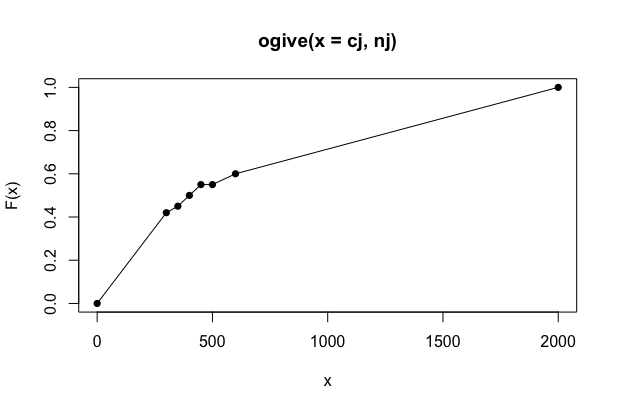
\includegraphics[scale=0.5]{Figures/R-ogive-plot.png}
\end{center}
\end{exemple}

\section{Exercices recommandés}
À compléter


\chapter{Estimation de données modifiées (12)}
\section{Point estimation}
\subsection{Définitions importante}
Un vocabulaire spécifique aux données modifiées est utilisé, soit

\begin{tabular}{|>{\bfseries} l |>{\em}l |p{3cm}|}
\hline
Définition	& Terme anglais & Explication \\
\hline	\hline
Tronquée à gauche	& left truncated at $d$ & si la valeur observée est plus basse dque $d$, elle n'est pas enregistrée \\
Tronquée à droite	& right truncated at $u$ & si la valeur observée est plus grande que $u$, elle n'est pas enregistrée \\
Censurée à gauche & left censured at $d$ & si la valeur observée est plus basse que $d$, on indique $d$ dans les données modifiées \\
Censurée à droite & right censored at $u$ & si la valeur observée est plus grande que $u$, on indique $u$ dans les données modifiées \\
\hline
\end{tabular}

\textbf{Note} : Il arrive aussi que les données soient \emph{shifted at $d$}, ce qui veut dire qu'on soustrait $d$ aux données (souvent en présence d'un déductible). 

\subsubsection{Notation}
\begin{enumerate}[label=\faAngleRight]
\item \blue{$y_1 < y_2 < ... < y_k$} : les $k$ valeurs uniques qui apparaissent dans l'échantillon.

\item \blue{$x_j$} : la $j$\up{e} données non-censurée qui apparait dans l'échantillon

\item \blue{$d_j$} : le montant auquel $x_j$ est tronquée. Si il n'y a pas de troncage, alors $d_j = 0$.

\item \blue{$u_j$} : la $j$ \up{e} données censurée qui apparait dans l'échantillon.

\item \blue{$r_j$} : nombre d'observations qui sont plus grandes ou égales à $y_j$ (\emph{risk set})
\begin{align*}
r_j = \text{\# of $x_i$} + \text{\# of $u_i$} - (\text{\# of $d_i$} \geq y_j)
\end{align*}

\item \blue{$s_i$} : nombre de décès au temps $i$.
\end{enumerate}

\subsubsection{Estimateur de Kaplan-Meier}
Cet estimateur est une version modifiée de l'estimateur de Nelson-\r{A}alen vu à la section \ref{subsec:nelson-Aalen}. Avec l'information des données et en utilisant la notation vue à la sous-section précédente, on peut estimer la fonction de survie empirique : 
\begin{equation}
\hat{S}_n(t) =
\begin{cases}
1		& , 0 \leq t < y_1 \\
\prod_{i=1}^{j-1} \left( \frac{r_i - s_i}{r_i} \right) & , y_{j-1} \leq t < y_j \quad j = 2, ..., k \\
\prod_{i=1}^{k} \left( \frac{r_i - s_i}{r_i}  \right) & t \geq y_k \\
\end{cases}
\end{equation}


\section{Espérance, Variance et et intervalle d'estimation}

\subsubsection{Contexte}
On s'intéresse à l'espérance et la variance de la fonction de survie $S_n$, qui suite une binomiale (i.e. $S_n(x) \sim Bin(n, S(x))$. Si on connaissait $S(x)$, on pourrait facilement déduire l'espérance et la variance avec les formules qu'on connaît. Toutefois, puisqu'on cherche souvent à estimer $S(x)$, il faudra aussi estimer l'espérance et la variance.

\hl{Section à compléter}


\section{Exercices recommandés}
À compléter



\part{Matière pour l'examen final}

\chapter{Continuous models (5)}

\section{Multiplication par une constante}
Soit $X$ la v.a. représentant les pertes et $\theta$ un paramètre d'échelle (\emph{scale parameter}). On peut définir la v.a. $Y$ par
\[Y = \theta X \]
Alors,
\begin{align*}
F_Y(y) 	 & = \prob{Y \leq y} \\ 
	& =\prob{\theta X \leq y} \\
	& = \prob{X \leq \frac{y}{\theta}} \\
	& = F_X \left( \frac{y}{\theta} \right) \\ \numberthis
\end{align*}
Et on peut aussi trouver que
\begin{align*}
f_Y(y) & = \derivee{y} F_Y(y) \\
	& = \derivee{y} \left\{ F_X \left( \frac{y}{\theta} \right)     \right\} \\
	& = \frac{1}{\theta} f_X \left( \frac{y}{\theta} \right) \\ \numberthis
\end{align*}

\paragraph{À noter} Si on doit appliquer une transformation impliquant une puissance (\emph{raising to a power}, voir section \autoref{sec:raise-to-power}), on applique cette dernière transformation avant d'appliquer le paramètre d'échelle $\theta$.


\section{Raising to a power}
% Label pour faire référence la section précédente.
\label{sec:raise-to-power}

Soit $X$ une v.a. représentant la perte avec une loi de probabilité quelquonque et la v.a. $Y$ tel que
\[Y = X^{\frac{1}{\tau}} \]
avec $\tau > 0$. On peut trouver $F_Y(y)$ ainsi que $f_Y(y)$ : 
\begin{align*}
F_Y(y) & = \prob{Y \leq y} \\
	& = \prob{ X^{\frac{1}{\tau}} \leq y} \\
	& = \prob{X \leq y^\tau} \\
	& = F_X \left( y^\tau \right) \\ \numberthis
\end{align*}
et
\begin{align*}
f_Y(y)	& = \derivee{y} F_y(y) \\
	& = \derivee{y}  F_X \left( y^\tau \right) \tau y^{\tau -1} f_X \left(y^\tau   \right) \\ \numberthis
\end{align*}

\paragraph{Note} On préfère toujours des paramètres positifs, donc on va ajuster les formules avec des constantes négatives dans certains cas.

\begin{exemple}[Notation dans le livre \emph{Loss Models}]
La notation utilisée par le livre est la suivante : 
\begin{enumerate}[label=\faAngleRight]
\item si $\tau > 0$ : \emph{transformed}
\item si $\tau =  -1$ : \emph{inverse}
\item si $\tau < 0$ et $\tau \neq 1$ : \emph{inverse-transformed}
\end{enumerate}
\end{exemple}

\section{Exponentiation}
Soit $X$ une v.a. représentant la perte. On définit $Y$ comme
\[Y = \exp(X)  \]
Alors, on trouve
\begin{align*}
F_Y(y)	& = \prob{Y \leq y } \\
	& = \prob{e^X \leq y } \\
	& = \prob{X \leq \ln y} \\
	& = F_x( \ln y) \\ \numberthis
\end{align*}
et 
\begin{align*}
f_Y(y)	& = \derivee{y} F_Y(y) \\
	& = \derivee{y} \left\{F_x( \ln y)   \right\} \\
	& = \frac{1}{y} f_X(\ln y) \\ \numberthis
\end{align*}

\paragraph{Note} La loi Log-Normale est en fait une transformation exponentielle de la Loi Normale.

\section{Lois mélanges}
On peut créer des lois mélanges. En effet, il arrive qu'on ait une distribution dont l'un des paramètres est lui-même distribué aléatoirement selon une autre distribution, tel que
\[ X | \Lambda \sim \text{une certaine loi}   \]
\[ \Lambda \sim \text{une autre loi (ou la même!)} \] 

On peut trouver les fonctions de densité et de répartition de ces différentes lois : 
\begin{equation}
f_X(x) = \int_{- \infty}^{\infty} f_{X|\Lambda}(x | \lambda) f_\Lambda(\lambda) d \lambda
\end{equation}
\begin{equation}
F_X(x) = \int_{- \infty}^{\infty} F_{X | \Lambda}(x | \lambda) f_\Lambda(\lambda) d \lambda
\end{equation}
De plus, on peut trouver l'espérance et la variance de ces lois mélanges avec les théorèmes de l'espérance et la variance conditionnelle : 
\begin{equation}
\esp{X} = \esp{ \esp{X | \Lambda} }
\end{equation}
\begin{equation}
Var(X) = \esp{Var(X | \Lambda)} + Var \left( \esp{X | \Lambda}   \right)
\end{equation}


\section{Frailty models}
%% À valider si c'est à l'examen!
\red{Est sur le syllabus des examens professionnels, mais ne semble pas être à l'étude pour le cours IARD1 ...} \\

Soit un paramètre $\Lambda > 0$ (\emph{frailty random variable}) qu'on va utiliser pour trvouer la \emph{hazard-rate} conditionnel $h_{X | \Lambda}$ tel que
\begin{equation}
h_{X | \Lambda}(x | \lambda) = \lambda a(x)
\end{equation}
où $a(x)$ est une fonction quelquonque et la distribution de $\Lambda = \lambda$ est connu. Alors, on peut trouver la fonction de survie de $S_{X | \Lambda}(x | \lambda)$ avec des des propriétés que l'on connait : 
\begin{align*}
S_{X | \Lambda}(x | \lambda) & = e^{- \int_{0}^{x} h_{X | \Lambda}(t | \lambda) dt} \\
	& = e^{- \lambda A(x)} \\
	& = M_\Lambda \left( - A(x) \right) \\
	& = \laplace_\Lambda \left( A(x) \right) \\
\end{align*}


\section{Splicing}
Soit $X_1, ..., X_k$ les différentes distributions que peut prendre la v.a. $X$ et $\alpha_i$ la probabilité que $X \sim X_i \quad , i = 1,2, ..., k$.  Pour $\sum_ \alpha = 1$, on a donc
\begin{align*}
f_X(x)	& = 
\begin{cases}
\alpha_1 f_1(x)	& , c_0 < x < c_1 \\
\alpha_2 f_2(x)	& , c_2 < x < c_2 \\
...							& \\
\alpha_k f_1(k)	& , c_{k-1} < x < c_k \\
\end{cases}
\end{align*}

\paragraph{Note} Dans un problème, on peut soit demander de calculer la fonction de répartition à un certain point, ou encore nous demander de trouver les coefficients $\alpha_i$ en connaissant les différentes fonctions de répartition et les probabilités rattachées.


\section{Exercices recommandés}
Les exercices recommandés dans le \emph{Loss Models, 4\up{th} edition} pour ce chapitre sont les suivants : 
\begin{enumerate}[label=\faAngleRight]
\item 5.1 à 5.6
\item 5.8 à 5.11
\item 5.17 à 5.19
\end{enumerate}



\chapter{Modèle de perte aggrégée (9)}

\section{Modèle composé (fréquence-sévérité) pour les pertes aggrégées}
On définit les variables aléatoires suivantes : 
\begin{enumerate}[label=\faAngleRight]
\item $S$ : Perte totale pour le portefeuille au complet ;
\item $N$ : Nombre de réclamations observées dans l'intervalle de temps. (\textbf{fréquence}) ;
\item $X_1, ..., X_n$ : Montant de perte relié à la $i$\up{e} réclamation (\textbf{sévérité}).\footnote{Les $X_i$ sont iid et indépendants de $N$.}
\end{enumerate}
On a donc
\[ S = X_1 + ... X_n  \]
et on peut trouver diverses quantités, tel que la fonction de répartition : 
\begin{equation}
F_S(x) = \sum_{n=0}^{\infty} F_X^{*n}(x) \prob{N = n}
\end{equation}
où $F_X^{*n} = \prob{X_1 + ... + X_n \leq n}$. \\

On peut aussi obtenir la fonction gnératrice des moments : 
\begin{equation}
\mathcal{M}_S(t) = \mathcal{P}_N \left( \mathcal{M}_X(t) \right) 
\end{equation}
L'espérance et la variance peuvent être obtenues avec les propriétés d'espérance et variance conditionnelle : 
\begin{align*}
\esp{S}	& = \esp{ \esp{S | N}} \\
	& = \esp{\esp{\sum_{i=1}^{n} X_i  }} \\
	& = \esp{\sum_{i=1}^{n} \esp{X_i}} \\
	& \overset{iid}{=} \esp{N \esp{X}} \\
	& = \esp{N} \esp{X} \\ \numberthis
\end{align*}

\begin{align*}
\variance{S}	& = \variance{\esp{S | N}}  + \esp{\variance{S | N}} \\
	& = \variance{\esp{\sum_{i=1}^{n} X_i}} + \esp{\variance{\sum_{i=1}^{n} X_i}} \\
	& \variance{ \sum_{i=1}^{n} \esp{X_i}} + \esp{\sum_{i=1}^{n} \variance{X_i}} \quad \text{, par indépendance des $X_i$} \\
	& \overset{iid}{=} \variance{N \esp{X}} + \esp{N \variance{X}} \\
	& = \esp{X}^2 \variance{N} + \esp{N} \variance{X} \\ \numberthis
\end{align*}


\section{Exercices recommandés}
Les exercices recommandés dans le \emph{Loss Models, 4\up{th} edition} pour ce chapitre sont les suivants : 
\begin{enumerate}[label=\faAngleRight]
\item 9.34 et 9.36
\end{enumerate}



\chapter{Frequentist estimation (13)}


\section{Méthode des moments}
On cherche à estimer les paramètres de la distribution de nos données, sachant que la distribution suit une loi quelconque. \\

Si on a $p$ paramètres à estimer, alors il faudra calculer les $p$ premiers moments empiriques de la distribution, soit
\begin{equation}
\hat{\mu}_k^\prime = \sum_{i=1}^{n} x_i^k
\end{equation}

Puis d'utiliser cette quantité empirique pour résoudre le système d'équation à $p$ inconnus tel que $\hat{\mu_k^\prime} = \mu_k^\prime$.

\section{Méthode des percentiles}
Pour un rappel sur les percentiles, voir la \autoref{sec:percentile}. Cette méthode est appelée en anglais \emph{percentile matching estimate}. \\

Un peu comme la méthode des moments, on utilise une quantité qu'on peut calculer empiriquement, soit la fonction de répartition empirique, pour pouvoir résoudre le système d'équations à $p$ variables tel que
\[F_n(\hat{\pi}_{g_i}) = g_i \]
où
\begin{enumerate}[label=\faAngleRight]
\item $\hat{\pi}_{g_i} = F_n^{-1}(g_i)$, $i = 1, ... ,p$
\item $F_n$ : la fonction de répartition empirique\footnote{L'estimation de la fonction de répartition empirique est couvert au \autoref{chap:estimation_Fn}.}
\item $p$ : nombre de paramètres de la distribution à estimer.
\end{enumerate}

\subsection{Smoothed empirical estimate}
Il arrive parfois que le percentile arrive entre 2 \emph{marche} de la fonction de répartition empirique. Dans cette situation, $\hat{\pi}_{g}$ doit être approximé de façon linéaire avec les statistiques d'ordre : 
\begin{equation}
\hat{\pi}_g = (1-h) X_{(j)} + h X_{(j+1)}
\end{equation}
où
\begin{enumerate}[label=\faAngleRight]
\item $j = \lfloor (n+1) g \rfloor$ et $h = (n+1) g - j$
\item $X_{(j)}$ la $j$\up{e} statistique d'ordre de l'échantillon empirique $X$.

\end{enumerate}






\section{Méthode du maximum de vraisemblance}
\subsection{Données complètes}
aussi appelé \emph{Maximum log-likelihood estimator (MLE)}. On cherche à estimer le paramètre $\hat{\theta}$ en maximisant la fonction de vraisemblance \footnote{Il arrive parfois que la seule façon de trouver le paramètre qui maximise $L(\theta)$ est en utilisant des \href{https://gitlab.com/vigou3/methodes-numeriques-en-actuariat}{méthodes numériques}}.

\begin{definition}[Fonction de vraisemblance]
La fonction de vraisemblance $L(\theta  | x)$ est la probabilité d'obtenir un échantillon $x_1, ..., x_n$ d'une distribution $f_X(x)$ ayant le vecteur de paramètres ${\theta}$. Alors,
\begin{equation}
\label{eq:fct_vraisemblance}
L(\theta)	= \prod_{i=1}^{n} f_X(x_i ; \theta)
\end{equation}
On peut aussi trouver la fonction de log-vraisemblance $\ell(\theta)$ (qui est souvent plus facile à dériver) : 
\begin{equation}
\label{eq:fct_log-vraisemblance}
\ell(\theta) = \sum_{i=1}^{n} \ln f_X(x_i ; \theta)
\end{equation}
\end{definition}
\paragraph{Estimation du paramètre $\theta$} On détermine l'estimateur du maximum de vraisemblance (\emph{MLE} en anglais)\footnote{L'abbréviation en français est MVE, mais on utilise surtout \emph{MLE} pour Maximum likelihood estimator.} tel qu'on maximise l'\autoref{eq:fct_vraisemblance}. Intuitivement, on va donc trouver le paramètre $\theta$ tel que
\[\derivee{\theta} L(\theta) = 0\]
Puisque la fonction de vraisemblance peut parfois être difficile à dériver, on utilise souvent la fonction de log-vraisemblance (\autoref{eq:fct_log-vraisemblance}) : 
\[\derivee{\theta} \ell(\theta) = 0\]
\paragraph{Estimation du vecteur de paramètres $\boldsymbol{\theta}$}
Si on doit estimer plusieurs paramètres pour la fonction $f_X$, on procède de la même façon, en dérivant partiellement la fonction de vraisemblance (ou log-vraisemblance) par rapport à chacun des paramètres et en posant ces dérivées égales à 0.



\subsection{Données groupées}
Lorsque les données sont groupées dans les intervalles $c_0 < c_1 < ... < c_k$, la fonction de vraisemblance $L(\theta)$ est différente. $X \sim Multinomiale(\matr{n}, \matr{p})$. Alors,
\begin{equation}
L(\theta) = \prob{n_1, n_2, ..., n_k ; \theta} = \binom{n}{n_1, ..., n_k} p_1^{n_1} ... p_k^{n_k}
\end{equation}
Dans le contexte de données groupées, on a que $p_j= \prob{X_j \in (c_{j-1}, c_{j})}$. Donc, la fonction de vraisemblance est
\[L(\theta) =  \prod_{j=1}^{n}  \left( F_X(c_{j} | \theta) - F_X(c_{j-1} | \theta) \right)^{n_j}   \]
Et la fonction de log-vraisemblance (en enlevant la constante combinatoire) est donc
\begin{equation}
\label{eq:log-vraisemblance_group}
\ell(\theta)  = \sum_{j=1}^{k} n_j \ln \left( F_X(c_{j} ; \theta) - F_X(c_{j-1} ; \theta) \right) \\
\end{equation}

\subsection{Données censurées}
Si une donnée est censurée, on l'interprète comme une donnée groupée dont l'intervalle va jusqu'à $\infty$. On remplace $f_X(x_j )$ par $1 - F_X(x_j )$.

\subsection{Données tronquées}
Si une donnée est tronquée, on a 2 options : 
\begin{enumerate}
\item On soustrait de chacune des observations le point de troncation $d$ ; 
\item \textbf{(Méthode plus souvent utilisée)} : On conditionne pour que les données sous le point de troncation $d$ ne soient pas considérées, i.e. on remplace $f(x_j | \theta)$ par $\frac{f(x_j | \theta)}{1 - F(d)}$. 
\end{enumerate}




\section{Calcul de la variance et intervalle de confiance}

\begin{definition}[Information de Fisher]

\begin{equation}
I(\theta) = -n \esp{\frac{\partial^2}{\partial \theta^2} \ln f_X(x ; \theta)} = n \esp{\left( \derivee{\theta} \ln f_X(x ; \theta) \right)^2}
\end{equation}
Il existe une autre version (plus générale) : 
\begin{equation}
I(\theta) = -\esp{\frac{\partial^2}{\partial \theta^2} \ell(\theta)} = \esp{\left( \derivee{\theta} \ell(\theta) \right)^2}
\end{equation}
\end{definition}







% Dernière section du chapitre
\section{Exercices recommandés}
Les exercices recommandés dans le \emph{Loss Models, 4\up{th} edition} pour ce chapitre sont les suivants : 
\begin{enumerate}[label=\faAngleRight]
\item Méthode des moments et percentiles : 13.1 à 13.22
\item \emph{MLE} : 13.30, 13.32, 13.33, 13.37, 13.38 à 13.40
\item 13.45 à 13.51
\item 13.54 à 13.57
\item 13.62 à 13.72
\item 13.74 
\end{enumerate}




\chapter{Estimation Bayésienne (15)}
\section{Définition de l'estimateur Bayésien}
\begin{definition}[Distribution \emph{a priori}]
Soit un paramètre $\theta$ d'une distribution quelconque. Afin de réaliser une estimation Bayésienne, on connaît \emph{a priori} la distribution que prend le paramètre $\theta$, qu'on dénote par $\pi(\theta)$. \\

Alors, notre distribution des pertes est conditionné par rapport à la valeur que $\theta$ prend (i.e. $f_{X|\Theta}$).
\end{definition}

\begin{definition}[Distribution \emph{a posteriori}]
La distribution \emph{a posteriori} nous permet de savoir avec quelle probabilité non-nulle notre paramètre $\theta$ peut prendre une certaine valeur, sachant qu'on a observé certains $x$, qu'on dénote comme $\pi_{\Theta | X}(\theta | x)$ : 
\begin{equation}
\label{eq:dist_posteriori}
\pi_{\Theta | X}(\theta | x) = \frac{f_{\Theta, X}(\theta, x)}{f_{X}(x)} = \frac{f_{X|\Theta}(x | \theta) \pi(\theta)}{\int f_{X|\Theta}(x | \theta) \pi(\theta) d \theta} 
\end{equation}
L'idée est de remplacer les différentes distributions dans l'\autoref{eq:dist_posteriori}, et en déduire une distribution avec une paramétrisation différente\footnote{Souvent, la distribution \emph{a posteriori} aura la même distribution que celle \emph{a priori}, mais avec des paramètres différents.}.
\end{definition}

\paragraph{L'estimateur Bayésien} L'estimateur Bayésien est défini comme l'espérance du paramètre $\theta$, sachant la distribution de $X$. En d'autres mots, on veut l'espérance de la distribution \emph{a posteriori} : 
\begin{equation}
\label{eq:estimateur_bayes}
\hat{\theta}_{BAYES} = \esp{\Theta | X}
\end{equation}

\paragraph{Propriétés de l'estimateur} Voici quelques propriétés importantes de l'estimateur : 
\begin{enumerate}[label = \faAngleRight]
\item $\hat{\theta}_{BAYES}$ est biaisé (comparativement à l'estimateur MLE qui est non-biaisé) ;
\item Par contre, l'estimateur Bayésien a une plus petite variance que l'estimateur MLE. On sacrifie donc le Biais pour diminuer la variance de l'estimateur ;
\item \textbf{Remarque} : Si $n$ est grand,  il peut être préférable d'utiliser l'estimateur MLE.
\end{enumerate}

\subsection{Estimation par simulation}
Une fois qu'on a développé et trouver la distribution \emph{a posteriori} de$\Theta | X$ (\autoref{eq:dist_posteriori}), alors on peut facilement simuler l'estimateur Bayésien :
\begin{enumerate}
\item 
\end{enumerate}


\begin{exemple}[Exemple avec la Loi de Poisson]
Soit $X | \Lambda \sim Pois(\Lambda)$ et $\Lambda \sim \Gamma(\alpha, \theta)$. Alors, on a la distribution \emph{a priori} suivante : 
\[\Lambda \sim \pi(\lambda) = \frac{\lambda^{\alpha -1}}{\Gamma(\alpha) \theta^\alpha} e^{-\lambda / \theta} \] 
Évidemment, on va s'attendre à ce que la distribution \emph{a posteriori} obéisse à une loi Gamma aussi. On a (avec $c(x)$ une constante) : 
\begin{align*}
\pi_{\Lambda | X}( \lambda | x) &  =c(x) \frac{\lambda^{\alpha -1} e^{-\lambda / \theta}}{\Gamma(\alpha) \theta^{\alpha}} \frac{\lambda^{\alpha} e^{-\lambda}}{x!} \\
& = k(x) \lambda^{x + \alpha - 1} e^{-\lambda\left( \frac{1}{\theta} + \lambda \right)} \\
\end{align*}
avec $c(x)$ et $k(x)$ des constantes uniquement fonction de $x$. \\

On trouve donc que $\pi_{\Lambda | X}( \lambda | x)  \sim \Gamma\left( \alpha' = x + \alpha, \beta' = \left(\frac{1}{\theta} + 1 \right)^{-1} \right)$

Puisque l'estimateur Bayésien est l'espérance de la distribution \emph{a posteriori}, on a
\begin{align*}
\hat{\lambda}_{BAYES} & = \esp{\Lambda | X} \\
& = \int \lambda \cdot \pi_{\Lambda | X}( \lambda | x) d \lambda \\
& = \alpha' \beta' \\
& = (x + \alpha) \left( \frac{\theta}{1 + \theta} \right) \\
\end{align*}
\end{exemple}

\begin{exemple}[Cas plus général ...]
On a le modèle suivant pour $X$, tel que
\begin{align*}
f_{X_1, ..., X_n | \Lambda}(x_1, ..., x_n | \lambda) & = \frac{\lambda^{x_1} e^{-\lambda}}{x_1 ! } ... \frac{\lambda^{x_n} e^{-\lambda}}{x_n !} \\
\end{align*}
Ainsi que la distriution \emph{a priori} telle que
\begin{align*}
\Lambda \sim \pi(\lambda) = \frac{\lambda^{\alpha -1}}{\Gamma(\alpha) \theta^{\alpha}} e^{-\lambda / \theta} \\
\end{align*}
Alors, la distribution \emph{a posteriori} est donc
\begin{align*}
f_{\Lambda | X}(\lambda | x)	& = c(x) \frac{\lambda^{\alpha-1}}{\Gamma(\alpha) \theta^{\alpha}} e^{-\lambda / \theta} \cdot \frac{\lambda^{x_1} e^{-\lambda}}{x_1 !} ... \frac{\lambda^{x_n} e^{-\lambda}}{x_n !} \\
& = k(x) \lambda^{\sum x_i + \alpha - 1} e^{-\lambda/ \theta} e^{-n \lambda} \\
& = k(x) \lambda^{\sum x_i + \alpha - 1} e^{-\lambda \left( \frac{1}{\theta} + n \right)} \\
\end{align*}
On déduit donc que la distribution \emph{a posteriori} obéit à une loi Gamma de paramètres $\alpha' = \sum x_1 + \alpha$ et $\beta' =\left( \frac{1}{\theta} + n \right)^{-1} = \frac{\theta}{1 + n \theta}$. Alors, on déduit facilement l'estimateur Bayésien : 
\begin{align*}
\hat{\lambda}_{BAYES} & = \alpha' \beta' \\
& =\frac{ \theta \left( \sum_{i=1}^{n} x_i + \alpha \right)}{1 + n \theta} \\
& =  \frac{n \theta}{1 + n \theta} \left( \frac{\sum_{i=1}^{n} x_i}{n} \right) + \frac{1}{1 + n \theta} (\alpha \theta) \\
& = \frac{n \theta}{1 + n \theta} \hat{\lambda}_{MLE} + \frac{1}{1 + n \theta} \underbrace{(\alpha \theta)}_{\text{Moy. distr. \emph{a priori}}} \\
\end{align*}
\paragraph{Remarque} On peut donc voir l'estimateur Bayésien comme une moyenne pondérée entre l'estimateur du maximum de vraisemblance et la moyenne de la distribution \emph{a priori}. Lorsque $n \to \infty$, l'estimateur Bayésien sera semblable à l'EMV.
\end{exemple}





\section{Intervalle de crédibilité}
L'intervalle de crédibilité\footnote{L'utilisation du terme crédibilité ici n'a aucun rapport avec la crédibilité utilisée dans le chapitre 17 du Loss Models.} est l'équivalent d'un intervalle de confiance qu'on utilise pour toutes les autres formes d'estimation vues auparavant.








\end{document}
